\documentclass[10pt]{article}

\usepackage{graphicx}
\usepackage{graphics}
\usepackage{multicol}
\usepackage{epsfig,amsmath,amsfonts}

\makeatletter                                   % Make '@' accessible. 
\oddsidemargin=0in                              % Left margin minus 1 inch.
\evensidemargin=0in                             % Same for even-numbered pages.
\marginparsep=0pt                               % Space between margin & text

\renewcommand{\baselinestretch}{1}              % Double spacing

\textwidth=6.5in                                % Text width (8.5in - margins).
\textheight=9in                                 % Body height (incl. footnotes)

\topmargin=0in                                  % Top margin minus 1 inch.
\headsep=0.0in                                  % Distance from header to body.
\skip\footins=4ex                               % Space above first footnote.
\hbadness=10000                                 % No "underfull hbox" messages.
\makeatother                                    % Make '@' special again.


\title{Bombilla: A Tiny Virtual Machine for TinyOS}
\author{Philip Levis\\pal@cs.berkeley.edu}
\date{}

\begin{document}

%\fontfamily{cmss}                               % Make text sans serif.
%\fontseries{m}                                  % Medium spacing.
%\fontshape{n}                                   % Normal: not bold, etc.
%\fontsize{10}{10}                               % 10pt font, 10pt line spacing 

\maketitle
\vspace{2in}
\begin{center}
Version 0.1\\
August 26, 2002
\end{center}

\fontfamily{cmr}                                % Make text Roman (serif).
\fontseries{m}                                  % Medium spacing.
\fontshape{n}                                   % Normal: not bold, etc.
\fontsize{10}{10}                               % 10pt font, 10pt line spacing


\thispagestyle{empty}
\newpage
\tableofcontents
\newpage

\section{Introduction}

Bombilla is a tiny bytecode interpreter that runs on top of
TinyOS. Because it presents a high-level communication-centric
interface, Bombilla's programs are very short; combined with a safe
execution environment, this makes mote reprogramming rapid and
error-free. Programs can self-propagate through a network; this makes
reprogramming mostly autonomous, as once a self-propagating capsule is
introduced, it will eventually install itself over the entire network.

Bombilla has multiple execution contexts; each runs in response to an
event, and they can interleave at instruction granularity. Bombilla
prevents race conditions by implicitly locking all shared state that
is used; as every resource is statically named and Bombilla programs
are short, the set of required locks can be quickly determined with a
full program analysis. Program writers can explicitly yield or release
locks to improve parallelism.

One goal of Bombilla is to provide a programming interface to motes
that is much simpler than TinyOS; a sense-and-send program can be as
few as six instructions in Bombilla, and Bombilla's error detection
mechanisms can help novice programmers find the bugs in their
programs.

\section{System Overview}

Bombilla is a set of TinyOS components that sit on top of several
system components, including sensors, the network stack, and
non-volatile storage (the ``logger''). Code is broken in {\bf
capsules} of 24 instructions, each of which is a single byte long;
larger programs can be composed of multiple capsules. In addition to
bytecodes, capsules contain identifying and version
information. Bombilla has two stacks: an operand stack and a return
address stack. Most instructions operate solely on the operand stack,
but a few instructions control program flow and several have embedded
operands. There are three execution contexts that can run concurrently
at instruction granularity. Bombilla provides both a built-in ad-hoc
routing algorithm (the {\tt send} instruction) as well as mechanisms
for writing new ones (the {\tt sendr} instruction).

\begin{figure}
\centering
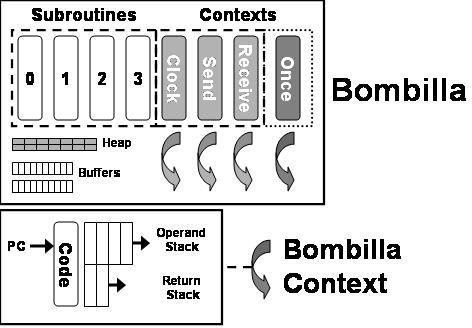
\includegraphics[scale=0.4]{fig/bombillamodel.jpg}
\caption{Bombilla Architecture and Execution Model: Capsules, Contexts, and Stacks}
\label{fig:exec}
\end{figure}


\begin{figure}
\begin{center}
\def\W{3.25in}

\begin{tabular}{|l|l|l|}\hline
basic   &{\tt 00iiiiii} & {\tt i} = instruction\\ \hline
m-class &{\tt 010iixxx} & {\tt i} = instruction, {\tt x} = argument \\ \hline
v-class &{\tt 011ixxxx} & {\tt i} = instruction, {\tt x} = argument \\ \hline
j-class &{\tt 10ixxxxx} & {\tt i} = instruction, {\tt x} = argument \\ \hline
x-class &{\tt 11xxxxxx} & {\tt i} = instruction, {\tt x} = argument\\ \hline
\end{tabular}

\caption{Bombilla Instruction Formats}
\label{fig:instr}
\end{center}
\end{figure}

\section{Architecture, Instruction Set, and Data Types}

Bombilla instructions hide the asynchrony (and oft-resulting race
conditions) of TinyOS programming. For example, when the {\tt send}
instruction is issued, Bombilla calls a command in the ad-hoc routing
component to send a packet. Bombilla suspends the context until a
message send complete event is received, at which point it resumes
execution. By doing this, Bombilla does not need to manage message
buffers -- the capsule will not resume until the network component is
done with the buffer. Similarly, when the {\tt sense} instruction is
issued, Bombilla requests data from the sensor TinyOS component and
suspends the context until the component returns data with an
event. This synchronous model makes application level programming much
simpler and far less prone to bugs than dealing with asynchronous
event notifications. Additionally, Bombilla efficiently uses the
resources provided by TinyOS; during a split-phase operation, Bombilla
does nothing on behalf of the calling context, allowing TinyOS to put
the CPU to sleep or use it freely.

Bombilla is a stack-based architecture. This allows a concise
instruction set; most instructions do not have to specify operands, as
they exist on the operand stack. There are five classes of Bombilla
instructions: basic, m-class, j-class, v-class, and x-class. Figure
\ref{fig:instr} shows the instruction formats for each class. Basic
instructions include such operations as arithmetic, halting, and
activating the LEDs on a mote. m-class instructions access message
headers; they can only be executed within the message send and receive
contexts. v-class instructions access the 16 word Bombilla
heap. j-class instructions are the two jump instructions, for loops
and conditionals. The one x-class instructions is {\tt pushc} (push
constant). All instruction classes except basic have embedded operands..

Bombilla's three principal execution contexts, illustrated in Figure
\ref{fig:exec}, correspond to three events: clock timers, message
receptions and message send requests.  Inheriting from languages such
as FORTH, each context has two stacks, an operand stack and a return
address stack. The former is used for all instructions handling data,
while the latter is used for subroutine calls. The operand stack has a
maximum depth of 16 while the call stack has a maximum depth of 8. We
have found this more than adequate for programs we have written.

There is an additional context, the ``once'' context. Unlike other
contexts, which run their capsules many times, this context only runs
its capsule once, when it is installed; this allows a user to
initialize state, adjust constants, or perform other operations that
only need a single execution.

There are three operands types: values, sensor readings, and
buffers. Some instructions can only operate on certain types. For
example, the {\tt putled} instruction expects a value on the top of
the operand stack. However, many instructions are polymorphic. For
example, the {\tt add} instruction can be used to add any combination
of the types, with different results. Adding buffers results in
appending the data in the second operand onto the first
operand. Adding a value to a message appends the value to the message
data payload. Sensor readings can be turned into values with the {\tt
cast} instruction.

Sensor readings are typed, and cannot be modified. For example, in
order to take an average over a set of readings, each reading must be
first be converted to a value; these values can then be averaged. Many
instructions (e.g. {\tt inv}) automatically cast sensor readings to
values. This ensures that a sensor reading variable has some meaning;
otherwise, it could express some arbitrary quantity. Adding two sensor
readings of the same type (e.g. magnetometer X-axis) produces a value,
and adding two sensor readings of different values is an error.

Buffers are also typed, and can hold up to ten values. A buffer can
only hold elements of one type, whether they be values or a certain
sensor type. An empty buffer has no type; the first element added will
set the type of the buffer. Buffers have several access instructions,
including {\tt bhead} (copy of the first element of the buffer onto
the operand stack), {\tt byank} (pull the nth element out of the
buffer and push it into the operand stack), and {\tt bsorta} (sort the
elements in ascending order.

There is a 16 word heap shared among the context. It can be accessed
with the {\tt setvar} and {\tt getvar} instructions, which have a
4-bit embedded operand.. This allows the separate contexts to
communicate shared state (e.g. sensor readings).

\subsection{Capsules and Execution}

Bombilla programs are broken up into capsules of up to 24
instructions. This limit allows a capsule to fit into a single TinyOS
packet. By making capsule reception atomic, Bombilla does not need to
buffer partial capsules, which conserves RAM. Every code capsule
includes type and version information. Bombilla defines four types of
code capsules: message send capsules, message receive capsules, timer
capsules, and subroutine capsules. Subroutine capsules allow programs
to be more complex than what fits in a single capsule. Applications
invoke and return from subroutines using the {\tt call} and {\tt
return} instructions. There are names for up to $2^{15}$ subroutines;
to keep Bombilla's RAM requirements small, its current implementation
has only four.

Bombilla begins execution in response to an event -- a timer going
off, a packet being received, or a packet being sent. Each of these
events has a capsule and an execution context. Control jumps to the
first instruction of the capsule and executes until it reaches the
{\tt halt} instruction. These three contexts can run
concurrently. Each instruction is executed as a TinyOS task, which
allows execution interleaving at an instruction
granularity. Additionally, underlying TinyOS components can operate
concurrently with Bombilla instruction processing. When a subroutine is
called, the return address (capsule, instruction number) is pushed
onto a return address stack and control jumps to the first instruction
of the subroutine. When a subroutine returns, it pops an address off
the return stack and jumps to the appropriate instruction.

\begin{figure}
\begin{center}
\scriptsize
\begin{tabular}{l}
\verb;getvar 0    # Get heap variable 0;\\
\verb;pushc 1     # Push one onto operand stack;\\
\verb;add         # Add the one to the stored counter;\\     
\verb;copy        # Copy the new counter value;\\
\verb;setvar 0    # Set heap variable 0;\\
\verb;pushc 7 ;\\     
\verb;and         # Take bottom three bits of counter;\\
\verb;putled      # Set the LEDs to these three bits;\\
\verb;halt;\\
\end{tabular}
\normalsize

\caption{Bombilla {\tt cnt\_to\_leds} -- Shows the bottom 3 bits of a counter on mote LEDs}
\label{fig:cnt}
\end{center}
\end{figure}


\begin{figure}
\begin{center}
\scriptsize
\begin{tabular}{l}
\verb;pushc 1     # Push one on the operand stack;\\
\verb;sense       # Read sensor 1 (light);\\
\verb;copy        # Copy the sensor reading;\\
\verb;getvar 0    # Get previous sent reading;\\
\verb;;\\
\verb;inv         # Invert previous reading ;\\
\verb;add         # Current - previous sent value;\\
\verb;copy        # 2 copies of difference on top of stack;\\
\verb;pushc 32    #;\\
\verb;;\\
\verb;gt          # Is current 32 greater than previous?;\\
\verb;swap        # Swap result with copy ;\\
\verb;pushc 32    #;\\
\verb;inv         #;\\
\verb;;\\
\verb;lt          # Is current 32 less than previous?;\\
\verb;or          # Either  32> or 32<;\\
\verb;jumps 15    # Jump to send;\\
\verb;halt;\\
\verb;;\\
\verb;copy        # Copy new value;\\
\verb;setvar 0    # Set current;\\
\verb;bpush0      # Push buffer 0 onto stack;\\
\verb;bclear      # Clear its contents;\\
\verb;;\\
\verb;add         # Add current reading to buffer;\\
\verb;send        # Send buffer;\\
\verb;halt;\\

\end{tabular}
\normalsize
\caption{Bombilla Program to Read Light Data and Send a Packet on Reading Change}
\label{fig:sense}
\end{center}
\end{figure}

The packet receive and clock capsules execute in response to external
events; in contrast, the packet send capsule executes in response to
the {\tt sendr} instruction. As {\tt sendr} will probably execute a
number of Bombilla instructions in addition to sending a packet, it can
be a lengthy operation. Therefore, when {\tt sendr} is issued, Bombilla
copies the message buffer onto the send context operand stack and
schedules the send context to run. Once the message has been copied,
the calling context can resume execution. The send context executes
concurrently to the calling context, preparing a packet and later
sending it. This frees up the calling context to handle subsequent
events -- in the case of the receive context, this is very important.

The constrained addressing modes of Bombilla instructions ensure a
context cannot access the state of a separate context. Every push and
pop on the operand and return value stack has bound checks to prevent
overrun and underrun. As there is only a single shared variable, heap
addressing is not a problem. Unrecognized instructions result in
simple no-ops. All bounds are always checked -- the only way two
contexts can share state is through {\tt gets} and {\tt
sets}. Nefarious capsules can at worst clog a network with packets --
even in this case, a newer capsule will inevitably be heard. By
providing such a constrained execution environment and providing
high-level abstractions to services such as the network layer, Bombilla
ensures that it is resilient to buggy or malicious capsules.

\subsection{Simple Programs}
\label{sec:sub:simple}

The Bombilla program in Figure \ref{fig:cnt} maintains a counter that
increments on each clock tick. The bottom three bits of the counter
are displayed on the three mote LEDs. The counter is kept as a value
which persists at the top of the stack across invocations. This
program could alternatively been implemented by using {\tt gets} and
{\tt sets} to modify the shared variable.  This code recreates one of
the simplest TinyOS applications, {\tt cnt\_to\_leds}, implemented in
seven bytes.

The Bombilla program in Figure \ref{fig:sense} reads the light sensor
on every clock tick. If the sensor value differs from the last sent
value by more than a given amount (32 in this example), the program
sends the data using Bombilla's built-in ad-hoc routing system. This
program is 24 bytes long, fitting in a single capsule.

\subsection{Capsule Injector}

\begin{figure}
\begin{center}
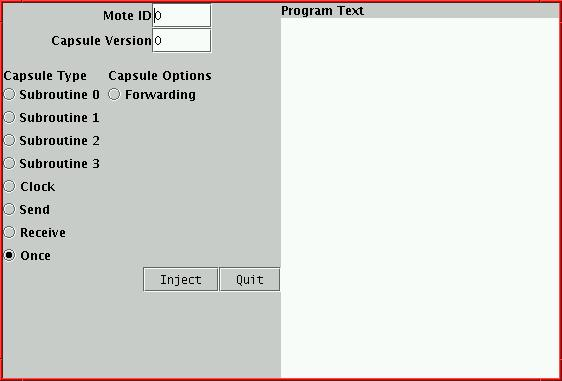
\includegraphics[width=2in]{fig/CapsuleInjector.jpg}
\caption{CapsuleInjector GUI}
\label{fig:capsuleinject}
\end{center}
\end{figure}

A tool is included in the TinyOS release to aid in the writing of
Bombilla programs: {\tt net.tinyos.vm\_asm.CapsuleInjector}. {\tt
CapsuleInjector} provides an interface for writing assembly programs
and sending them to a mote connected to a PC; if the capsule is marked
self-forwarding, it will then start propagating into the network.

One must set the destination mote ID of the capsule packet (important
when using a GenericBase) and the version number of the
capsule. Version numbers are explained in Section \ref{sec:viral};
Bombilla only installs a capsule if its version number is higher than
the one it currently has.

If the program has an error (e.g. a v-class instruction without a
specified operand), {\tt CapsuleInjector} does not send out a packet.

\section{Synchronization}

Bombilla interleaves the execution of its contexts at instruction
granularity. The presence of a 16-word shared heap means that if
different contexts communicate or share variables (e.g. an aggregated
sensor reading), race conditions can easily occur. As the program
running on a mote is the combination of possibly forwarding capsules,
applications can go through transient states of partial installation,
making programmer efforts (e.g. a spin loop) ineffectual.

Bombilla therefore uses an implicit locking scheme, so that
programmers are assured that there will be no race conditions in their
programs. Experienced programmers can relax the locking requirements
to improve parallelism.

\subsection{Model}

In this section, we define the sychronization model, which is based on
five abstractions: \emph{handlers, invocations, resources, scheduling
points} and \emph{sequences}. We describe how we discover the
resources used by an invocation, and how invocation communicate their
resource requirements to the runtime system.

A \emph{handler} is a function that is executed in response to some
event. An \emph{invocation} represents a particular execution of a
handler in response to an event. At any time, invocations are in one
of four states: \emph{waiting} (for resources), \emph{suspended}
(waiting for an operation to complete), \emph{ready} (can execute),
\emph{running} (executing). We say that an invocation that is ready or
running is \emph{active}.

A \emph{resource} is a shared piece of state that a handler requires
access to -- examples are a variable, a disk arm, or a sensor.
Resources can only be held by invocations.

A handler contains a number of \emph{scheduling points} at which it can be
suspended and gain or lose resources (and resources cannot be acquired
anywhere but at scheduling points). Scheduling points are the handler's
entry and exit points, and some subset of its operations which we call
\emph{scheduled operations}. An invocation goes through two states during
execution of a scheduled operation: first, the invocation is suspended
awaiting the completion of the operation; second, the invocation is
waiting for the resources it wishes to gain to become
available. Either of these two phases may be trivial: a {\tt yield}
operation completes immediately but may wait for some resources, a
message send does not complete immediately but, if it is not waiting
for any resources, will not wait. A \emph{sequence} is any code path
between two scheduling points which does not include another
scheduling point.

The model for resource acquisition and release is as follows: before
an invocation can start execution, it must acquire all resources it
will need during its lifetime. At each subsequent scheduling point,
the invocation can release a set $R$ of resources before suspending
execution, and acquire a set $A$ of resources before resuming. To
prevent deadlock, we require $A
\subseteq R$ (we prove below that this condition is sufficient for building
deadlock-free schedulers). Finally, when an invocation exits it must
release all held resources. Note that we do not guarantee any atomicity
between two invocations of the same handler.

To preserve safety, the static analysis of a handler's resource usage
and the runtime system must guarantee that an invocation holds all
resources at the time(s) at which they are accessed and that the
intersection of the resources held by any two invocations is empty. We
restrict our invocation model to considering a static number of
resources, and require operations to explicitly name the resources
they use so that we can easily analyse handlers at compile (or load)
time. Resource discovery must be conservative to preserve correctness.

\subsection{Bombilla Implementation}

We implemented this syncronization model in Bombadillo. Each
Bombadillo context is an invocation, and capsules are implicitly
broken up into sequences. Bombadillo maintains two queues of
invocations: ready and waiting. Whenever Bombadillo installs a new
capsule, it performs a static full-program analysis to generate the
acquire sets of its invocation start points. Without requiring any
annotation from a programmer, Bombadillo runs invocations atomically
while allowing parallelism. Programmers can improve the degree of
parallelism by yielding resources at scheduling points.

Bombadillo invocations are broken into sequences by scheduling point
instructions. When a context executes one of these instructions, the
Bombadillo runtime examines the current release set of the issuing
context and releases the locks on the indicated resources. Bombadillo
then checks the waiting queue to see if any contexts have been made
runnable by the release of these locks. When the scheduling point
instruction completes, Bombadillo checks the acquire set of the
context to see if it can be made active; if so, the context acquires
its locks and Bombadillo places it on the ready queue. If the context
cannot be made active, Bombadillo places it on the waiting queue.

\begin{figure}
\centering
\tiny
\begin{tabular}{|l|l|}\hline
\verb;pushc 3  #                   ;&\verb; pushc 3 ;\\
\verb;unlock   # Add lock 3 to R,A ;&\verb; unlockb   # Add locks 0,1 to R,A;\\
\verb;pushc 2  #                   ;&\verb; pushc 12 ;\\
\verb;punlock  # Add lock 2 to R   ;&\verb; punlockb  # Add locks 2,3 to R;\\
\verb;sense    # Yield             ;&\verb; sense     # Yield;\\ \hline

\end{tabular}
\caption{Sample Bombilla Unlocking}
\label{fig:locks}

\end{figure}

Bombadillo defines its scheduling point instructions to be those that
trigger split-phase operations in TinyOS. This includes acquiring
sensor data ({\tt sense}), sending packets ({\tt send, sendr, uart}),
and accessing non-volatile flash memory storage ({\tt logr, logw,
logwl}). Additionally, there is a {\tt yield} instruction, which is
effectively a split-phase operation that immediately completes. Locks
are added to a context's release set with the {\tt unlock} instruction
-- by default, the set is empty. {\tt unlock} also adds the lock to
the context's acquire set. For a lock to be released, but not
re-acquired, a context much use the {\tt punlock} (unlock permanent)
instruction. The {\tt unlock} and {\tt punlock} instructions affect
individual locks, enumerated by an operand; the {\tt unlockb} and {\tt
punlockb} instructions use the operand as a bitmask for locks to be
released. Locks are not released until a scheduling-point instruction
is executed. Figure \ref{fig:locks} contains two sample Bombadillo
instruction sequences that demonstrate resource unlocking.

Release and acquire sets are atomically handled by Bombadillo. A
context does not acquire any locks in its acquire set unless it can
acquire all of them, and acquires them atomically. Similarly, release
sets are released atomically. This, combined with monotonically
decreasing lock sets, ensures the system is deadlock free.

\section{Viral Programming}
\label{sec:viral}

Bombilla code capsules can be marked ``forwarding.'' The code
forwarding system triggers roughly every 700 milliseconds; it takes a
rough estimate of the network's business, and probabilistically
decides whether it will forward a capsule. Capsules are forwarded more
often in a quiet network than in a busy one. If Bombilla decides to
forward a capsule, it chooses one at random and checks if it the
forwarding bit is set; if so, it transmits the capsule on an AM
broadcast.

Every capsule has a version number. When Bombilla hears a capsule
broadcast, it checks if the capsule is newer than the one currently
installed; if so, Bombilla halts execution of that context and
installs the new capsule.

Our first implementation of the VM had an explicit caspule forwarding
system (the {\tt forw} instruction); experimental results showed this
to be a terrible idea, as programs could very easily saturate the
network unknowingly. We therefore adopted this simple probabilistic
model. It is by no means perfect; for example, even if every mote in
the network is running the same capsule, they will continue to forward
it indefinitely. We are currently exploring more efficient code
propagation mechanisms.

\section{Error State}

Bombilla has an error state, which can help users debug their
programs. If a program triggers an error (for example, by trying to
add incompatible sensor readings, or by overflowing the operand
stack), Bombilla halts execution on all contexts. Then, every second,
it blinks all of the LEDs and sends a packet containing debugging
information over the UART. The packet contains the offending context
identifier, the capsule it was executing, the instruction that caused
the error, and the error code. Error codes can be found in
{\tt tos/lib/Bombilla.h}. They are:

\begin{verbatim}
typedef enum {
  BOMB_ERROR_TRIGGERED                =  0,
  BOMB_ERROR_INVALID_RUNNABLE         =  1,
  BOMB_ERROR_STACK_OVERFLOW           =  2,
  BOMB_ERROR_STACK_UNDERFLOW          =  3, 
  BOMB_ERROR_BUFFER_OVERFLOW          =  4,
  BOMB_ERROR_BUFFER_UNDERFLOW         =  5,
  BOMB_ERROR_INDEX_OUT_OF_BOUNDS      =  6,
  BOMB_ERROR_INSTRUCTION_RUNOFF       =  7,
  BOMB_ERROR_LOCK_INVALID             =  8,
  BOMB_ERROR_LOCK_STEAL               =  9,
  BOMB_ERROR_UNLOCK_INVALID           = 10,
  BOMB_ERROR_QUEUE_ENQUEUE            = 11,
  BOMB_ERROR_QUEUE_DEQUEUE            = 12,
  BOMB_ERROR_QUEUE_REMOVE             = 13,
  BOMB_ERROR_QUEUE_INVALID            = 14,
  BOMB_ERROR_RSTACK_OVERFLOW          = 15,
  BOMB_ERROR_RSTACK_UNDERFLOW         = 16, 
  BOMB_ERROR_INVALID_ACCESS           = 17,
  BOMB_ERROR_TYPE_CHECK               = 18,
  BOMB_ERROR_INVALID_TYPE             = 19,
  BOMB_ERROR_NOSUCHLOCK               = 20
} BombillaErrorCode;
\end{verbatim}

The Bombilla error packet has the following payload:

\begin{verbatim}
typedef struct BombillaErrorMsg {
  uint8_t context;
  uint8_t reason;
  uint8_t capsule;
  uint8_t instruction;
} BombillaErrorMsg;
\end{verbatim}

%\appendix

%\section{Source Files}

%There are many.

\end{document}
